\section{Antecedentes Generales}

\subsection{ALMA Common Software}
El ALMA Common Software(ACS) es la infraestructura de software, con una arquitectura distribuida e integrada, en donde se manejan todos los procesos del observatorio, desde la captura de los requerimientos para la observación hasta la entrega de los datos capturados \cite{Chiozzi2002}.

Una de las características de ACS es su carácter distribuido, posibilitando que la funcionalidad del sistema pueda implementarse en diferentes lugares geográficos.

Esto hace que ACS sea un sistema heterogéneo, donde diferentes máquinas (hardware) pueden ejecutar software en distintos sistemas operativos y lenguajes de programación. 
El objetivo de un sistema de estas características es que la comunicación entre clientes y servidores sea transparente, independiente de la arquitectura. Esta filosofía de desarrollo se basa en la separación entre la funcionalidad y la arquitectura técnica.
\\
\\
El propósito del \textit{framework} ACS es:
\begin{itemize}
\item Proveer un modelo de programación, para asegurar que una misma función pueda ser desarrollada y ejecutada de la misma forma en cualquier plataforma de desarrollo.
\item Provee interfaces para ser implementadas.
\end{itemize}

ACS provee una filosofía de desarrollo orientado a objetos y los servicios básicos para el cómputo distribuido.

Dentro de estos servicios se encuentran:

\begin{itemize}
\item Invocación remota de objetos transparente.
\item Manejo distribuido de errores y alarmas
\item Manejo distribuido de reporte de eventos (\textit{logging})
\end{itemize}


El \textit{framework} ACS está basado en CORBA\citep{Chiozzi2002}, y está construido en base a código libre.

\subsection{Logs}
\subsubsection{Definición de Log}
Un log es un registro o bitácora que indica la actividad de un sistema. Estos registros o eventos son posteriormente almacenados y tienden a responder el qué, el dónde, el cuándo de un evento particular del sistema \citep{ESOLOG}.


\begin{lstlisting}[label={lst:xml}, caption=Ejemplo un evento XML de log, language=XML]
<Debug TimeStamp="2002-10-7T13:44:16.530"
Host="te1.hq.eso.org" Process="baciTestServer" Thread="main"
Context="" File="baciTestClassImpl.cpp" Line="205"
Routine="BaciTestClass::~BaciTestClass">
    Great debug message!
</Debug>
\end{lstlisting}

Los archivos de Logs son fuentes de valiosa información acerca del estado de un sistema, o de un conjunto de sistemas interconectados. En el listing~\ref{lst:xml} se puede ver un ejemplo de un registro.

Los Logs a procesar son documentos en formato XML. Estos archivos contienen registros que indican información acerca del estado del sistema en forma de eventos. Los eventos, a su vez, contienen datos específicos que describen los detalles asociados al evento en cuestión. Por ejemplo, el instante de tiempo donde ocurre el evento, la máquina que origina, el proceso asociado, entre otros, y además de una descripción en lenguaje natural generada por un programador. 

Todos estos eventos están originalmente clasificados por un tipo que indica el grado de severidad del incidente. Por ejemplo, \textit{Error} , \textit{Warning}, \textit{Info}, \textit{Debug}, \textit{Critical}, etc. \citep{ESOLOG}.


\subsection{Pre-procesamiento de datos}

\subsubsection{Documentos legibles por máquinas}
Uno de los mayores problemas en los archivos de logs es que no están diseñados para el procesamiento automático, sino para ser interpretados por operadores humanos. Por lo tanto, es difícil generar un mecanismo automático para clasificar estos eventos en forma sistemática.


\subsubsection{Tratamientos de texto para los eventos}
Uno de los problemas para poder realizar clasificaciones es que casi todos los eventos son diferentes y es necesario agruparlos según criterios para reducir el número de estos.


Varios de los sistemas de predicción necesitan identificadores numéricos para caracterizar cada tipo de error\citep{Salfner2008a}. En algunos sistemas los eventos incorporan un identificador, y otros simplemente incorporan únicamente información detallada para cada evento, por lo que es necesario realizar algunas de las siguientes operaciones:

\begin{itemize}
\item Separar atributos de cada evento.
\item Remover números en los mensajes.
\item Eliminar atributos vacíos.
\item Transformar el tiempo a formato UNIX
\item \textit{Stemming} de palabras, (reducción a a la raíz de las palabras)
\item Eliminación de conectores en mensajes.
\end{itemize}


Posteriormente de haber tratado los eventos, un algoritmo de clasificación de texto puede generar \textit{clusters}. Algunos de los algoritmos usados para realizar clasificación de documentos de texto son:

\begin{itemize}
\item \textbf{Distancia de Levenshtein}: Este algoritmo calcula la distancia de dos textos, según el mínimo de operaciones requeridas para poder igualar ambos textos. Este valor es útil para poder comparar el parecido de dos mensajes de evento.
\item \textbf{Kmeans - IDF}: Este algoritmo combina dos conceptos diferentes el primero es la matriz inversa de frecuencia de palabras, en otras palabras, la frecuencia de cada termino en un documento, este documento puede ser un mensaje de un evento. El segundo algoritmo kmeans, puede relacionar y agrupar estas frecuencias para determinar clusters con frecuencias similares de los clusters, este algoritmo requiere un tratamiento extra, eliminando conectores y aplicando stemming.
\item \textbf{Locality-sensitive hashing algorithms}: Este tipo de algoritmos permite reducir la dimensionalidad de los datos. Al generar aproximaciones es posible realizar agrupaciones y comparar la similitud entre dos mensajes. Esta clase de algoritmos son utilizados para crear huellas digitales de documentos de video y audio, entre otras aplicaciones.  
\end{itemize}

\subsection{Procesamiento de datos}
Luego de haber pre-procesado los registros, es posible realizar el procesamiento de minería de datos para la búsqueda de patrones. Uno de los algoritmos posibles es:
\subsubsection{SVM}
Las Máquinas de Vectores de Soporte (SVM) abordan problemas de clasificación lineal, mediante la búsqueda de la superficie óptima de separación de dos clases. La superficie óptima, maximiza la distancia entre las dos clases, utilizando los datos más cercanos (vectores de soporte) para construir dicha superficie, como se describe en la Figura \ref{fig:svm} \cite{Cortes1995}. Cuando el problema es no lineal se realiza una proyección de los datos de entrada hacia un espacio llamado ''espacio de características'', generalmente de alta dimensión. Siempre existe un espacio, por más alta que sea su dimensión, en el que es posible encontrar un hiperplano lineal que separa dos clases, como lo muestra la Figura \ref{fig:svm}.

\begin{figure}[H]
\centering
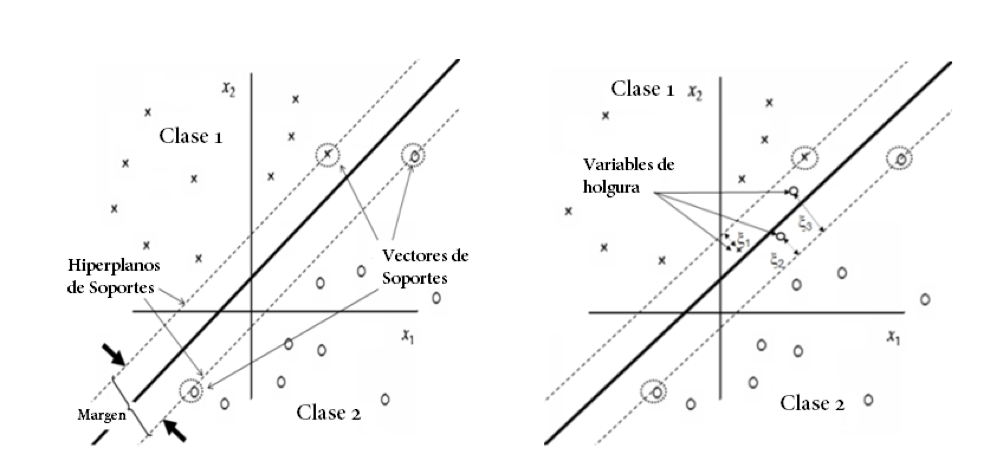
\includegraphics[scale=0.9]{img/svm}
\caption{Hiperplano lineal de separación de dos clases: (\textbf{a}) Margen máximo (\textbf{b}) Margen blando. Los datos destacados con círculos, son vectores de soporte}
\label{fig:svm}
\end{figure}
\newpage
Los parámetros del hiperplano lineal (w, b) se obtienen mediante un algoritmo de optimización que encuentra la mayor distancia (margen) respecto de los vectores de soporte\cite{Scholkopf2001}. Se definen los hiperplanos de apoyo que se muestran en la Figura \ref{fig:svm} (a). Por su parte, la Figura \ref{fig:svm} (b) muestra la situación de margen blando, o sea cuando se permite que algunos puntos crucen los hiperplanos de soporte. Las variables de holgura, son términos que indican en qué medida un punto se encuentra en el lado equivocado de su respectivo hiperplano de soporte. Para resolver problemas no lineales, se utiliza el ''truco del kernel''\cite{Scholkopf2001}. La función de transformación, llamada kernel, proyecta el espacio de entrada en el espacio de características, como se puede observar en la Figura \ref{fig:svm2}.


\begin{figure}[H]
\centering
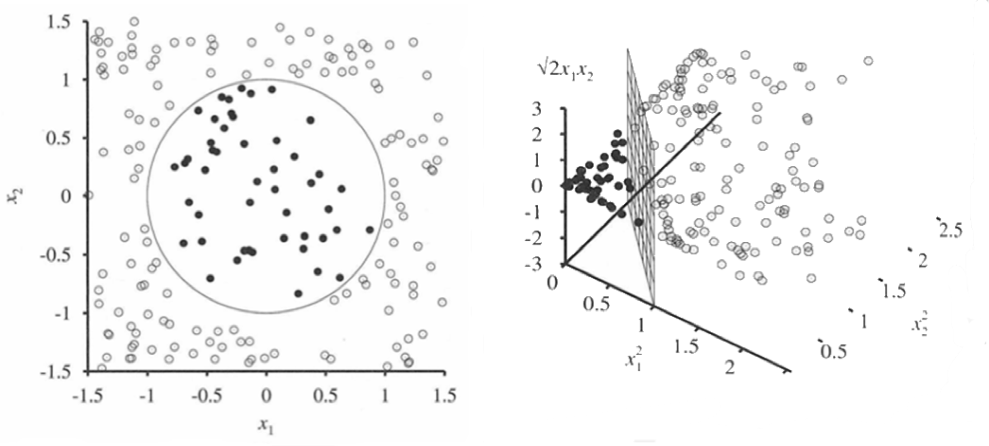
\includegraphics[scale=0.8]{img/svm2}
\caption{Efecto de la asignación del espacio de entrada en un espacio de características dimensional superior, donde es posible un plano de separación lineal.
}
\label{fig:svm2}
\end{figure}

